\chapter{Grundlagen}

% Grundlagen:


% - TrackSort Schüttgutsortierung
% - Kalman Filter
% - NN
% 	- RNN
% 	- LSTM

In diesem Kapitel soll eine kurze Einführung in die für das Verständnis der restlichen Arbeit benötigten Themengebiete gegeben werden.
Primär sollen zunächst allgemein neuronale Netze und einige ihrer speziellere Aspekte betrachtet werden 
bevor ein kurzer Blick auf das bei den Experimenten verwendete Schüttgutsortiersystem \textit{TableSort} geworfen wird. 

\section{Das Kalman-Filter}
Als Kalman-Filter bezeichnet man ein mathematisches Verfahren mit dem Messfehler in realen Messwerten reduziert werden können und nicht messbare Systemgrößen geschätzt werden können. 


[vergangene, aktuelle und zukünftige Systemzustände schätzen]
[Einschränkung Linearität (Extended Kalman) und Gauß rauschen]

Der Zustand des Systems zum Zeitschritt \(t\) wird als \(y_t\) und die Messung im Zeitschritt \(t\) als \(z_t\) bezeichnet.

\begin{equation}
	y_t = A y_{t-1} + w, 	w \sim N(0, Q)
\end{equation}

\begin{equation}
	z_t = H y_{t} + v, 	v \sim N(0, R)
\end{equation}

Dabei ist \(A\) die Zustandsübergangsmatrix, die den Übergang von einem Zustand in den nächsten beschreibt.
\(H\) ist die Messmatrix, die beschreibt wie Messungen aus dem Zustand entstehen und Q und R sind die Kovarianzmatrizen des Systemrauschens beziehungsweise des Messrauschens. 

Das Kalman-Filter funktioniert mittels abwechselnd ausgeführter \textit{predict} und \textit{update} Schritte.

\begin{equation}
\hat{y}'_t = A \hat{y}'_{t-1}
\end{equation}

\begin{equation}
	\hat{P}'_t = A \hat{P}'_{t-1} A^\textit{T} + Q
\end{equation}





\section{Neuronale Netze}

Als Neuronale Netze  % beziehungsweise \textit{künstliche neuronale Netze}, wie sie manchmal korrekter genannt werden, 
bezeichnet man in der Informatik Systeme aus künstlichen Neuronen, die heute eine wichtige Rolle im Feld des maschinellem Lernen einnehmen.
Manchmal werden sie korrekter als \textit{künstliche neuronale Netze} bezeichnet um sie von \textit{natürlichen neuronalen Netzen} 
wie dem menschlichen Gehirn zu unterscheiden, nach deren biologischem Vorbild sie inspiriert sind.
  %sind vom biologischen Vorbild des menschliche Ge

Die Grundsteine des Feldes wurde bereits 1943 von Warren McCulloch und Walter Pitts gelegt, 
die in ihrem Paper \cite{mcculloch1943logical} ein Neuronenmodell vorschlugen, mit dem sich logische arithmetische Funktionen berechnen lassen. 
Nach einer Periode von relativ geringer Aufmerksamkeit der wissenschaftlichen Gemeinschaft während den 1970ern und folgenden Jahrzehnten 
haben einige bahnbrechende Ergebnisse um das Jahr 2010, unter anderem im Feld der Spracherkennung, das Interesse an dem Feld wieder entfacht. 


% Nachdem jedoch Marvin Minsky und Seymour Papert zeigten, dass einzelne Perzeptrons nicht in der Lage sind linear nicht separierbare Probleme zu lösen sank das Interesse an dem Feld.

\subsection{Perzeptron}
Die kleinste Einheit eines neuronalen Netzes ist das Perzeptron, wie es 1958 von Frank Rosenblatt beschrieben wurde \cite{rosenblatt1958perceptron}.
Es ist eine Art künstliches Neuron, dass eine Reihe an Eingaben entgegen nimmt und einen einzelnen Wert $o$ ausgibt.

\todo{Darstellung des Perzeptrons}

Die einzelnen Eingaben $x_i$ haben jeweils eine Gewichtung $w_i$.
Es existiert ein sogenannter Schwellwert oder \textit{bias}, der normalerweise 
durch eine zusätzliche Eingabe $x_{m+1}$ mit dem Wert $+1$ und dem dazugehörigen Gewicht $w_{m+1}$ modelliert wird.
Den Ausgabewert $y$ erhält man dadurch, dass man die gewichteten Eingaben aufsummiert und in die Aktivierungsfunktion des Perzeptrons gibt.
Ein Überblick über verschiedene Aktivierungsfunktionen ist unter \ref{activationfuncs} zu finden.

Mathematisch ist die Ausgabe eines Perzeptrons also wie folgt definiert:

\begin{equation}
	y = \phi ( \sum_{i= 0}^{m} w_i x_i)
\end{equation}

Beim Lernen werden die Gewichte der einzelnen Eingaben so an gepasst, dass die gewünschte Ausgabe erreicht wird.
Ein einzelnes Perzeptron mit zwei Eingängen kann zur Darstellung der logischen Operatoren AND, OR und NOT genutzt werden

Letztendlich ist ein solches Perzeptron jedoch nur ein linearer Klassifikator und kann somit zum Beispiel den XOR Operator nicht auflösen.
Dies zeigten Marvin Minksy und Seymour Papert 1969 in einflussreichen Buch \textit{Perceptrons} \todo{quelle}
\todo{Linear Trennbares / Nicht-linear Trennbares Problem (AND vs XOR)}

Um solche, nicht linear-separierbare Probleme zu lösen müssen mehrere Schichten an Neuronen kombiniert werden.

\subsection{Aktivierungsfunktionen}
\label{activationfuncs}
Es gibt verschiedene Aktivierungsfunktionen, die für den Einsatz in neuronalen Netzen in Frage kommen.
Sie sind von essenzieller Wichtigkeit, da ohne eine Nicht-Linearität das Netz in eine einfache Regression kollabiert.

Eine Aktivierungsfunktion sollte leicht abzuleiten sein, 
da dies im Rahmen des Backpropagation Algorithmus häufig geschieht und sonst beträchtlicher Rechenaufwand entsteht.

Einige häufig verwendete Aktivierungsfunktionen sollen hier vorgestellt werden.
Jede dieser Funktionen stellt eine Nicht-Linearität dar und nimmt eine einzelne Zahl, wendet eine bestimmte, festgelegte mathematische 
Operation auf diese an und gibt das Ergebnis zurück.

\begin{description}
	\item[Sigmoid-Funktion] \hfill \\
		\begin{equation}
			f(x) = \frac{1}{1 + e^x} = \frac{e^x}{e^{x + 1}}
			\label{func:Sigmoid}
		\end{equation}
		\begin{equation}
			f'(x) = f(x) * (1 - f(x))
		\end{equation}
		Die mathematische Form der Sigmoid Aktivierungsfunktion ist in Abbildung \ref{sigmoidFunc} zu sehen.
		Sie bildet die reellen Zahlen $\mathbb{R}$ auf das Intervall $(0,1)$ ab. 
		Für betragsmäßig größer werdende negative Zahlen nähert sich der Rückgabewert $0$ an,
		ebenso wie für größer werdende positive Zahlen sich der Rückgabewert an $1$ annähert.

		Die Sigmoid Funktion ist eine historisch häufig genutze Funktion, da sie das Verhalten eines natürlichen Neurons,
		der biologischen Motivation für künstliche Neuronen, gut nachbildet:
		komplette Inaktivität eines Neurons bei Ausgabe 0 bis zum feuern mit maximaler Frequenz bei Ausgabe 1.

		In der Praxis jedoch haben sich einige Nachteile der Sigmoid Funktion gezeigt, weshalb sie quasi nicht mehr genutzt wird.
		Der gewichtigste von diesen ist, dass ihre Ableitung bei großen Beträgen beinah $0$ ist.
		Dies führt dazu, dass während der Ausführung des Backpropagation-Algorithmus beinah keine Änderungen passieren und dementsprechend das Netz sehr langsam lernt.
		
		\begin{figure}
			\centering
			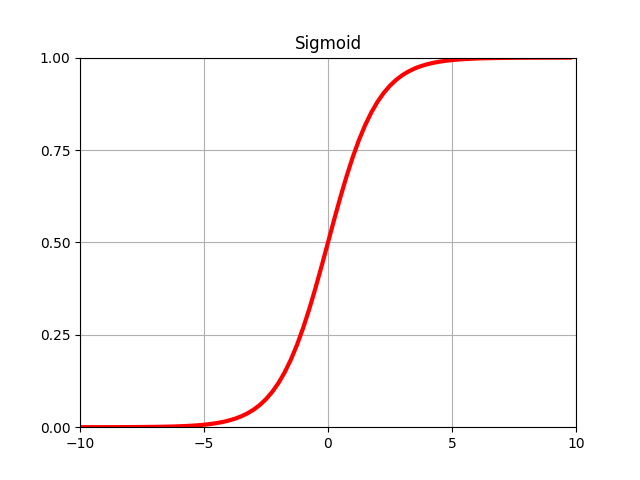
\includegraphics[width=0.618\textwidth]{Sigmoid}
			\caption{Plot der Sigmoid Funktion}
			\label{sigmoidFunc}
		\end{figure}
		  


	\item[TanH] \hfill \\
		\begin{equation}
			f(x) = \tanh(x) = \frac{e^x - e^{-x}}{e^x + e^{-x}}
		\end{equation}
		\begin{equation}
			f'(x) = 1 - f(x)^2
		\end{equation}
		Die tanh Aktivierungsfunktion ist in Abbildung \ref{tanhfunction} dargestellt.
		Im Gegensatz zur Sigmoid Funktion bildet sie die reellen Zahlen $\mathbb{R}$ auf das Intervall $(-1, 1)$ ab.
		Weil sie zentriert um den Nullpunkt ist, wird sie bei realen Anwendungen der Sigmoid Funktion vorgezogen.
		Das Saturationsproblem der Sigmoid Funktion besteht jedoch immer noch.
		\begin{figure}
			\centering
			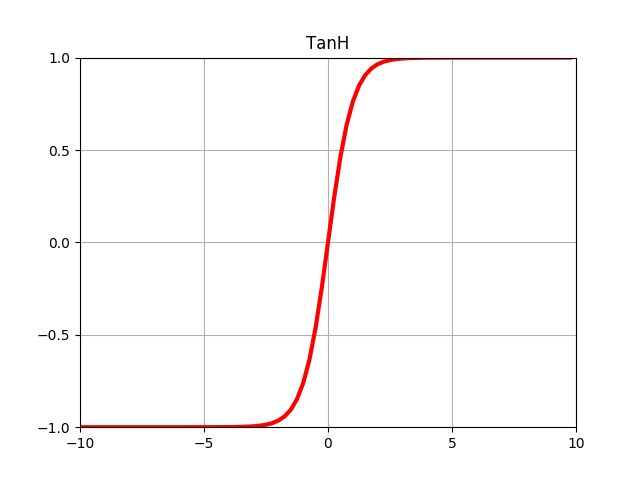
\includegraphics[width=0.618\textwidth]{Tanh}
			\caption{Plot der Tanh Funktion}
			\label{tanhfunction}
		\end{figure}
	
	\item[ReLU] \hfill \\
		\begin{equation}
			f(x) = max(0, x)
		\end{equation}
		\begin{equation*}
			f'(x) = \begin{cases}
			0 &\text{, falls $x < 0$}\\
			1 &\text{, falls $x > 0$}
			\end{cases}
		\end{equation*}
		Abbildung \ref{reluoutput} zeigt den Plot einer \textit{Rectified Linear Unit}, oder kurz ReLU.
		Die Aktivierung von ReLUs ist ein einfacher Schwellwert, der weit weniger rechenintensiv ist, als die aufwendigen Exponenzialfunktionen von Sigmoid und tanh.
		In der Praxis hat sich gezeigt zudem gezeigt, dass ReLus deutlich schneller konvergieren als Sigmoid- oder tanh-Neuronen. 
		Krizhevsky et al. haben in ihrem Paper\cite{NIPS2012_4824} einen Geschwindigkeitsgewinn um Faktor 6 feststellen können.
		Ein Problem, das mit ReLUs jedoch existiert ist, dass einzelne Neuronen während dem Training "absterben" können.
		Diese Neuronen sind dann für jeden beliebigen Input inaktiv und können nie wieder etwas zur Ausgabe des Netzes beitragen.
		Durch die Wahl einer geeigneten Lernrate oder den Einsatz sogenannter Leaky ReLUs lässt sich dies jedoch vermeiden.
		Leaky ReLUs haben im Gegensatz zu normalen ReLUs eine kleine positive Steigung im negativen Bereich.
		\begin{equation}
			f(x) = \begin{cases}
				x &\text{, falls } x  >  0\\
				0.01 x &\text{, falls } x  \leq  0
			\end{cases}
		\end{equation} 

		\begin{figure}
			\centering
			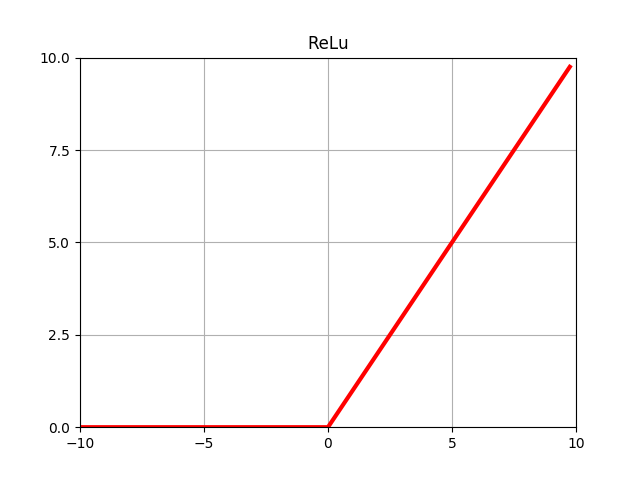
\includegraphics[width=0.618\textwidth]{ReLu}
			\caption{Plot der Ausgabe einer ReLUs}
			\label{reluoutput}
		\end{figure}



\end{description}

\begin{figure}[h]
    \centering
    \begin{subfigure}[t]{0.3\textwidth}
		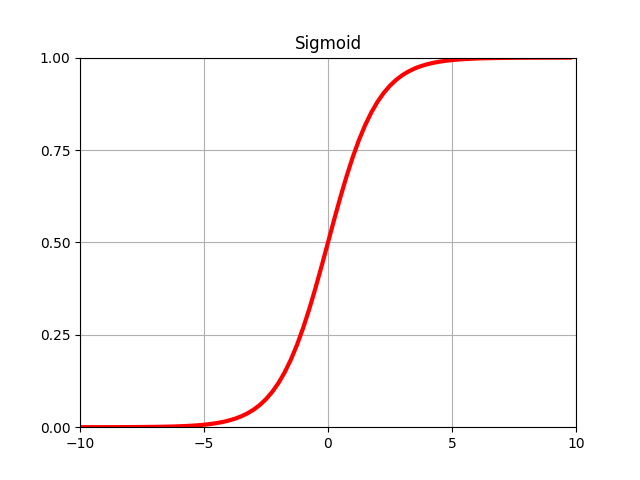
\includegraphics[width=\textwidth]{Sigmoid}
		\caption{Sigmoid Funktion}
    \end{subfigure}
    \begin{subfigure}[t]{0.3\textwidth}
		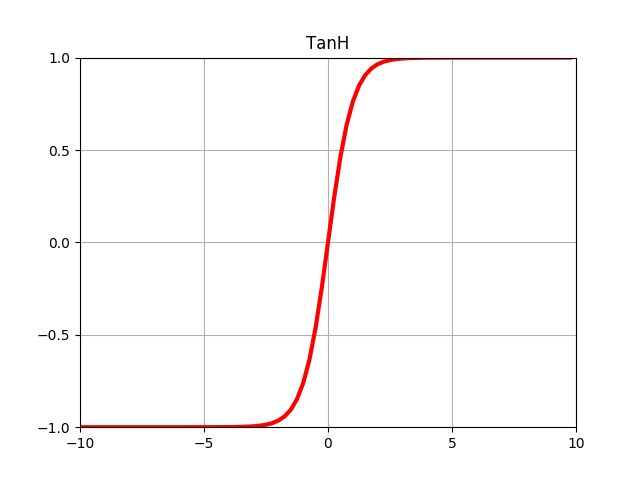
\includegraphics[width=\textwidth]{Tanh}
		\caption{TanH Funktion}
    \end{subfigure}
    \begin{subfigure}[t]{0.3\textwidth}
        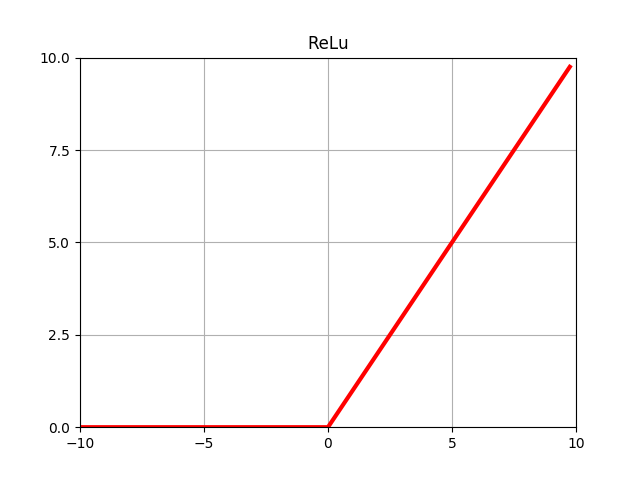
\includegraphics[width=\textwidth]{ReLu}
        \caption{ReLU}
    \end{subfigure}
    \caption{Häufig verwendete Aktivierungsfunktionen}
    \label{eval:function}
\end{figure}


\subsection{Feedforward Netze}

\textbf{absatz über Feedforward Netze. Basic}
Als Feedforward Netz bezeichnet man ein neuronales Netz, zwischen dessen Knoten keine Kreise oder Schleifen existieren.
Die Informationen wandert in der Verarbeitungsrichtung von den Eingabeknoten zu den Ausgabeknoten.
Für gewöhnlich sind die einzelnen Knoten in Schichten, sogenannten Layern, organisiert.
Die Neuronen eines einzelnen Layers sind meist 
Die Eingabe wird in ein Input Layer eingeben.

~~~~~~~~~~
- Outputlayer: Verschiedene Aktivierungsfunktionen:
. Linear für regression, z.B. Softmax für Wahrscheinlichkeitsverteilung Softmax
[One Hot encoding?]

\subsection{Backpropagation}

\todo{ein Absatz über lernen mit dem Backpropagation Algorithmus}
Der Backpropagation Algorithmus ist ein Verfahren mit denen künstliche neuronale Netze in der Lage sind komplizierte Zielfunktionen einzulernen.
Es ist eine Methode, bei der effizient der Gradient der Fehlerfunktion in Abhängigkeit vom Gewicht der einzelnen Kanten im Netz bestimmt werden kann,
was dann für einen Gradientenabstieg verwendet werden kann. 

\begin{itemize}
	\item Nur supervised learning: Gradient der Fehlerfunktion wird benötigt => Tatsächliches Ergebnis muss bekannt sein.
	\item "Finden einer Funktion, die am besten die Inputs auf die outputs mapt"
\end{itemize}

\subsection{Overfitting}

\todo{Absatz zu Overfitting}
Overfitting:
	Wenn das System schlechter darin wird zu generalisieren: (von bekanntem auf unbekanntes schließen/Schlechte Prediktion)
	Erkennen die Performance auf dem Trainingsset weiterhin besser wird, aber die Performance auf dem Testset schlechter wird.
	z.B. wenn Rauschen als teil der zugrundeliegenden Struktur interpretiert wird.

Gegenteil von Underfitting, wenn das Modell nicht ausreichend komplex ist um die zugrundeliegende Struktur der Daten abzubilden. 
Beispiel underfitting: Lineares Modell auf nicht-lineare Daten fitten.

\begin{figure}
	\missingfigure{Overfitting example}
	% \includegraphics[width=\textwidth]{TrackSortPic}
	\caption{Beispiel für Overfitting}
	% \todo{Quelle Bild!}
	\label{fig:overfitting}
\end{figure}

Methoden um Overfitting zu vermeiden:
Mehr Trainingsdaten (z.B. durch Data-Augmentation)
Regularisierung (L1, L2 (siehe unten), dropout für Classifier(?))


\subsection{Regularisierung}

Als Regularisierung bezeichnet man eine Technik, die benutzt wird um ein Modell von Overfitting abzuhalten.
Sie wird in der Hoffnung angewendet, dass das Modell mit Regularisierung besser generalisiert als ohne.

Die Grundidee ist, dass zur loss function ein Regularisierungsterm hinzugefügt wird, 
der die Kosten basierend auf der Komplexität des Systems erhöht.

\begin{equation}
	\min_f \sum\limits_{i=1}^{m} V(f(\vec{x}_i), \vec{y}_i) + \lambda R(f)
\end{equation} 

Dabei ist $V$ die loss function, beispielsweise \textit{Mean-Square-Error} oder \textit{Mean-Absolute-Error}.
$n$ ist die Anzahl der Feature-Label-Paare,
$x_i$ und $y_i$ sind die einzelnen Eingabefeatures und das dazugehörige Label.
Die Funktion $f$ ist in unserem Fall das neuronale Netz, das die Features entgegen nimmt.
$\lambda$ ist ein Parameter, der die Gewichtung des Regularisierungsterm festlegt.
Wählt man diesen Parameter zu klein, so kann es sein, dass das Modell immer noch overfittet.
Wählt man ihn zu groß so kann es sein, dass das Modell das Problem nicht mehr korrekt abbildet und es zu Underfitting kommt.
Der Regularisierungsterm $R$ wird so gewählt, dass er die Komplexität der Funktion $f$ wiederspiegelt.
Beispiele für $R$ wären zum Beispiel die L1- oder die L2-Regularisierung die jeweils mit der L1 beziehungsweise mit der L2 Norm arbeiten.

Ein gutes Maß für die Komplexität eines neuronalen Netzes sind die Gewichte zwischen den Neuronen.

Formel für MSE mit L1 Regularisierung findet man in \ref{eqn:MSE-L1}.
\begin{equation} \label{eqn:MSE-L1}
	J(X, Y) = \frac{1}{m} \sum_{i=1}^{m} (\vec{y}^{(i)} - \hat{\vec{y}}^{(i)})^2 + \sum_{j} \sum_{k} (|\mat{W}_{j,k}|)
\end{equation} 

\todo{absatz zu regularization - L1, L2, (L0 und warum man es nicht benutzt?)}


\section{TableSort System}

[Viel stuff über das TableSort System]

kleiner, experimenteller Bandsortierer \cite{doll2015}

\begin{figure}
	% \missingfigure{Bild von TablesortSystem}
	\includegraphics[width=\textwidth]{TrackSortPic}
	\caption{TableSort Schüttgutsortiersystem [TODO Quelle]}
	% \todo{Quelle Bild!}
	\label{tablesortsystemimage}
\end{figure}